\documentclass[a4paper]{article}
\usepackage{tikz}
\usetikzlibrary{decorations}
\usetikzlibrary{decorations.pathmorphing, arrows.meta}
\usetikzlibrary{calc}
\usepackage{apacite}
\usepackage{tabularx}
\usepackage{siunitx}
\usepackage{amsmath}
\usepackage{rotating}
\usepackage{colortbl}
\usepackage[absolute]{textpos}


\begin{document}


\begin{titlepage}
    

    \title{\textbf{How does the moment of inertia affect the period of Maxwell's Wheel? \\ \small Physics HL Internal Assesment}}
    \author{Zhou Changhui}
    \date{\today}
    \maketitle
    %\tableofcontents
\end{titlepage}

\section{Introduction and background knowledge}

\section{Hypothesis and reasoning}

\begin{figure}[ht]
    \centering
    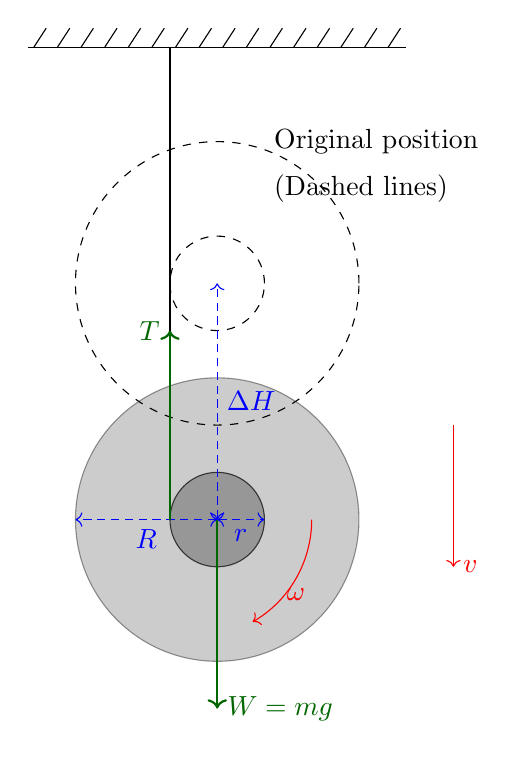
\begin{tikzpicture}[scale = 0.6] % Energy analysis tikzpic 
        \coordinate (O) at (0, 0);
        \draw[fill = gray, opacity = 0.4] (O) circle (3);
        \draw[fill = gray, opacity = 0.7] (O) circle (1);
        \draw[dashed] (0, 5) circle (3);
        \draw[dashed] (0, 5) circle (1);
        \node[right] at (1, 8) {Original position};
        \node[right] at (1, 7) {(Dashed lines)};
        \draw (-4, 10) -- (4, 10);
        \foreach \x in {-3.75, -3.25, ..., 3.75} 
            \draw[xshift = \x cm] (0.13, 10.4) -- (-0.13, 10);
        \draw[thick] (-1, 4) -- (-1, 10); 

        % Lengths
        \draw[<->, densely dashed, blue] (0, 0) -- (1, 0) node[midway, below, scale = 1] {$r$};
        \draw[<->, densely dashed, blue] (0, 0) -- (-3, 0) node[midway, below, scale = 1] {$R$};
        \draw[<->, densely dashed, blue] (0, 0) -- (0, 5) node[midway, right, scale = 1] {$\Delta H$};

        % Kinetics
        \draw[->, red] (5, 2) -- (5, -1) node[right, scale = 1] {$v$};
        \draw[->, red] (2, 0) arc (0: -60: 2.5) node[midway, right, below, scale = 1] {$\omega$};

        % Forces
        \draw[->, black!60!green, thick] (-1, 0) -- (-1, 4) node[above, left, scale = 1] {$T$};
        \draw[->, black!60!green, thick] (0, 0) -- (0, -4) node[below, right, scale = 1] {$W = mg$};
    \end{tikzpicture}
    \caption{Model of a Maxwell's Wheel}
    \label{fig.maxwellwheel}
\end{figure}

As is shown in Figure \ref{fig.maxwellwheel}, the Maxwell's wheel mainly consists of three parts: a wheel of radius $R$, an axle of radius $r$, and a string. Aside from friction, two forces are acting on the pendulum: the tension from the string and the gravitational force. During the entire process, the gravitational potential energy converts to kinetic energy of the wheel. 

The downward movement and the upward movement is basically symmetric, so only the downward reaction needs algebraric analysis.

Since the wheel is not in equilibrium, its hard to analyze the magnitude of tention $T$. However, the problem can be tackled using conservation of energy.

Due to the negeligibility of friction, we can assume that all the gravitational potential energy lost is converted to the kinetic energy. Or more specificly, the sum of the translational kinetic energy and rotational kinetic energy should equal to the loss in gravitational potential energy. Or formally,

\begin{equation}
    mg\Delta h = \frac{1}{2}m v^2 + \frac{1}{2} I \omega ^2
\end{equation}


where $I$ is the moment of inertia of the entire wheel. 

Moreover, using the definition of velocity and angular velocity, the following identites can be derived,

\begin{equation}
    \dfrac{\mathrm{d}\Delta H}{\mathrm{d}t} = v
\end{equation}

\begin{equation}
    \omega r = v
\end{equation}

\begin{equation}
    \Delta H(0) = 0
\end{equation}

Therefore

\begin{equation}
    mg\Delta H = \frac{1}{2}m v^2 + \frac{1}{2} \frac{I}{r^2} v ^2
\end{equation}

After moving and combining the terms

\begin{equation}
    \frac{2mg\Delta H}{m+\frac{I}{r^2}} = (\dfrac{\mathrm{d}\Delta H}{\mathrm{d}t})^2
\end{equation}

Moving ${\mathrm{d}\Delta H}/{\mathrm{d}t}$ to the left size and make its index $1$,

\begin{equation}
    \dfrac{\mathrm{d}\Delta H}{\mathrm{d}t} = \sqrt{\frac{2mg}{m+\frac{I}{r^2}}} \Delta H ^ {0.5}
\end{equation}

This is a simple ODE, with the help of formula (4), we can get that,

\begin{equation}
    \Delta H(t) = \dfrac{mg}{2m+\frac{2I}{r^2}} t^2
\end{equation}

The downward movement terminates when $\Delta H(t) = l$, which means 

\begin{equation}
    t_{down} = \sqrt{\dfrac{(2m+\frac{2I}{r^2})l}{mg}}
\end{equation}

The entire period of the Maxwell's Wheel is 

\begin{equation}
    T = 2t_{down} = 2\sqrt{\dfrac{(2m+\frac{2I}{r^2})l}{mg}}
\end{equation}

which can be re-written as 

\begin{equation}
    T^2 = 8l\dfrac{(m+\frac{I}{r^2})}{mg}
\end{equation}

From this formula, the hypothesis can be derived: \textbf{$T$ increases as $I$ increases. $T^2$ and $I$ has a linear relationship.}

\section{Experiment design}

\subsection{Variables} 

\begin{itemize}
    \item Independent variable: 
    \item Dependent variable: 
    \item Controlled variables: The material, mass and size of the plate and magnets. The length of the string. The mass, radius and length of the axle, etc.
\end{itemize}

\subsection{Materials}

\begin{itemize}
    \item[*] 2 Iron stands (height $\approx \SI{50}{cm}$)
    \item[*] 2 Cotton strings (length $\approx \SI{70}{cm}$)
    \item[*] 1 Acrylic disc (radius $\approx \SI{10}{cm}$, mass $\approx \SI{110}{g}$)
    \item[*] 16 Magnets (radius $\approx ??aa$, mass $\approx ??aa$)
    \item[*] 1 Force gauge ($\SI{50}{N}$)
    \item[*] 1 Tape rule
    \item[*] 1 Electric balance
    \item[*] 1 Vernier caliper  
\end{itemize}

\subsection{Setup diagram}

\begin{figure}[ht]
    \centering
    
    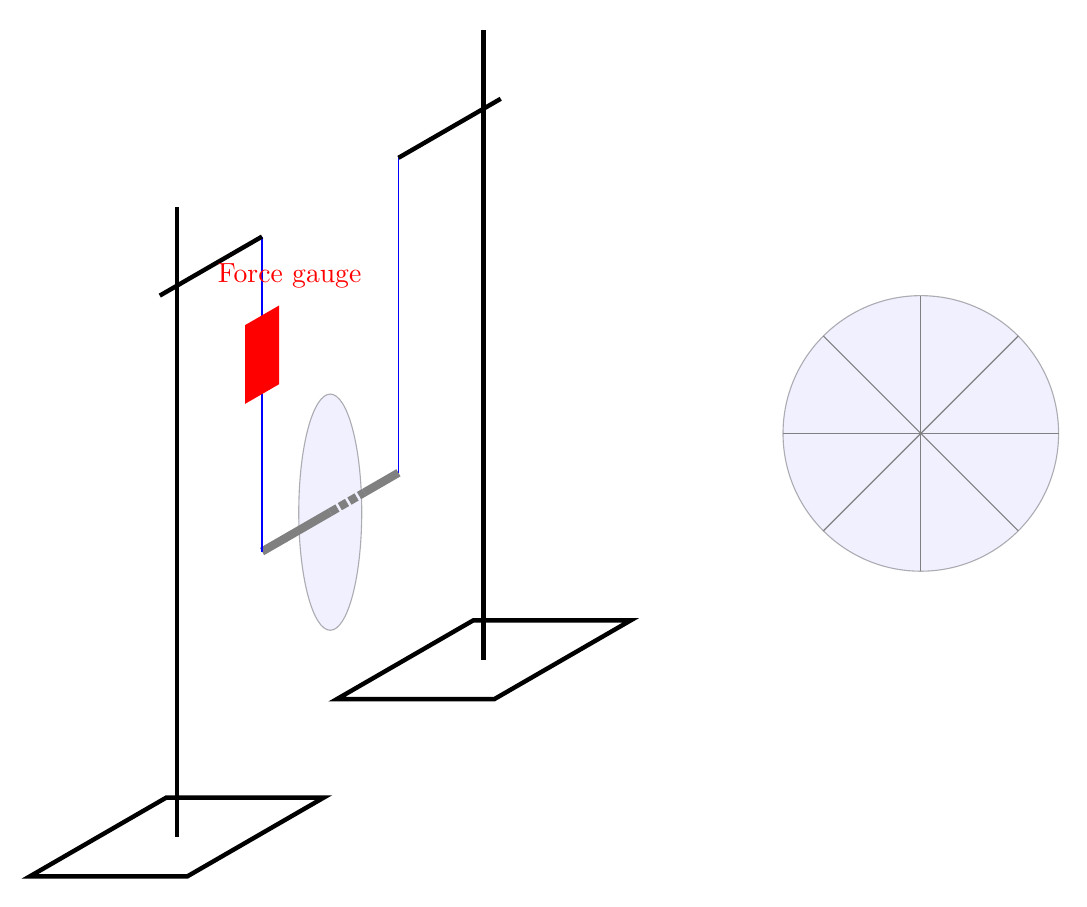
\begin{tikzpicture}[scale = 0.5]
    % No I think this is stupid
    
    % The acrylic plate 
        \draw[fill=blue!20, opacity=0.3, even odd rule] (0,0) ellipse (0.8 and 3);
        \coordinate (P) at ($(0,0) - (30:2)$);
        \coordinate (Q) at ($(0,0) + (30:2)$);
        \draw[line width=3pt, gray] (P) -- (0,0);
        \draw[densely dotted, line width = 3pt, gray] (0,0) -- ($(0,0) + (30:1)$);
        \draw[line width=3pt, gray] ($(0,0) + (30:1)$) -- (Q);
        \draw[blue, semithick] (P) -- ($(P) + (0, 8)$);
        \draw[blue, semithick] (Q) -- ($(Q) + (0, 8)$);
        \draw[black, ultra thick] ($(P) + (0, 8)$) -- ($(P) + (0, 8) - (30:3)$);
        \draw[black, ultra thick] ($(Q) + (0, 8)$) -- ($(Q) + (0, 8) + (30:3)$);
        \coordinate (R) at ($(P) + (0, -6) - (30:2.5)$);
        \coordinate (S) at ($(Q) + (0, -6) + (30:2.5)$);
        \draw[black, ultra thick] ($(P) + (0, 10) - (30:2.5)$) -- (R);
        \draw[black, ultra thick] ($(Q) + (0, 10) + (30:2.5)$) -- (S);
        \draw[black, ultra thick] ($(R) + (30: 2) + (2, 0)$) -- ($(R) + (30: 2) - (2, 0)$) -- ($(R) - (30: 2) - (2, 0)$) -- ($(R) - (30: 2) + (2, 0)$) -- cycle;
        \draw[black, ultra thick] ($(S) + (30: 2) + (2, 0)$) -- ($(S) + (30: 2) - (2, 0)$) -- ($(S) - (30: 2) - (2, 0)$) -- ($(S) - (30: 2) + (2, 0)$) -- cycle;
        \coordinate (X) at ($(P) + (0, 5)$);
        \fill[red] ($(X) + (0, 1) + (30: 0.5)$) -- ($(X) + (0, 1) - (30: 0.5)$) -- ($(X) - (0, 1) - (30: 0.5)$) -- ($(X) - (0, 1) + (30: 0.5)$) -- cycle;
        \node[red] at ($(X) + (0.7, 2)$) {Force gauge};
        
        \coordinate (O) at (15, 2);
        \draw[fill=blue!20, opacity=0.3] (O) circle (3.5);
        \draw[gray] ($(O) - (0 : 3.5)$) -- ($(O) + (0 : 3.5)$);
        \draw[gray] ($(O) - (45 : 3.5)$) -- ($(O) + (45 : 3.5)$);
        \draw[gray] ($(O) - (90 : 3.5)$) -- ($(O) + (90 : 3.5)$);
        \draw[gray] ($(O) - (135 : 3.5)$) -- ($(O) + (135 : 3.5)$);
        %\draw[black, ultra thick]
    \end{tikzpicture}

    \label{fig.setupdiagram}
\end{figure}

\end{document}